\documentclass[10pt]{article}
\newcommand{\figpaperwidth}{152mm}
\newcommand{\figpaperheight}{72mm}
\usepackage{amsmath}
\usepackage{pgfplots}
\pgfplotsset{compat=1.18}
\usetikzlibrary{arrows.meta,calc}
\setlength{\paperwidth}{\figpaperwidth}\setlength{\paperheight}{\figpaperheight}
\setlength{\pdfpagewidth}{\paperwidth}\setlength{\pdfpageheight}{\paperheight}
\setlength{\oddsidemargin}{-1in}\setlength{\topmargin}{-1in}
\setlength{\headheight}{0pt}\setlength{\headsep}{0pt}\setlength{\footskip}{0pt}
\setlength{\textwidth}{\paperwidth}\setlength{\textheight}{\paperheight}
\setlength{\parindent}{0pt}\pagestyle{empty}
\definecolor{dblue}{RGB}{31,95,153}
\definecolor{dorange}{RGB}{194,94,0}
\definecolor{dgray}{RGB}{110,110,110}
\begin{document}
\centering
\begin{tikzpicture}[font=\small]
\pgfplotsset{
  base/.style={width=58mm, height=46mm, scale only axis, font=\small,
    line width=0.8pt, grid=major, grid style={black!15},
    tick label style={font=\footnotesize},
    label style={font=\footnotesize},
    every axis plot/.append style={line width=1.0pt, mark size=2.0pt},
    xtick={20,50,100,200,400}, xticklabels={20,50,100,200,400},
    minor xtick={30,40,60,70,80,90,150,250,300,350},
    log ticks with fixed point}}

% (a) R against S_local, both families
\begin{loglogaxis}[base, name=a,
  xlabel={$S_{\mathrm{local}}$}, ylabel={$R=|E_{z,X}|/B_{\mathrm{up}}^{2}$},
  xmin=10, xmax=420, ymin=0.04, ymax=1.6,
  title={\footnotesize (a) rate against local Lundquist number},
  legend style={at={(0.02,0.03)}, anchor=south west, font=\footnotesize,
    draw=black!30, fill=white, fill opacity=0.9, text opacity=1}]
  % Orszag-Tang, admitted: data/scaling.csv
  \addplot[dgray, mark=square*, mark options={fill=dgray}]
    coordinates {(66.75,0.7736) (137.9,0.3403) (281.0,0.1602)};
  % island coalescence, this work, common window p in [0.30,0.38]
  \addplot[dblue, mark=*, mark options={fill=dblue}]
    coordinates {(18.14,0.076516) (40.23,0.12241) (126.36,0.11316)};
  % slope -1 guide through the first OT point
  \addplot[dorange, dashed, forget plot, domain=40:340, samples=2]
    {51.64/x};
  \legend{Orszag--Tang, island coalescence}
  \node[font=\footnotesize, text=dorange, anchor=west] at (axis cs:150,0.52)
    {$\propto S^{-1}$};
\end{loglogaxis}

% (b) the product R*S, constant exactly when R ~ 1/S
\begin{semilogxaxis}[base, name=b, at={($(a.east)+(20mm,0)$)}, anchor=west,
  xlabel={$S_{\mathrm{local}}$}, ylabel={$R\,S_{\mathrm{local}}$},
  xmin=10, xmax=420, ymin=0, ymax=50,
  title={\footnotesize (b) the product $R\,S_{\mathrm{local}}$}]
  \addplot[dgray, mark=square*, mark options={fill=dgray}]
    coordinates {(66.75,43.72) (137.9,41.70) (281.0,40.82)};
  \addplot[dblue, mark=*, mark options={fill=dblue}]
    coordinates {(18.14,1.388) (40.23,4.925) (126.36,14.30)};
  \node[font=\footnotesize, text=dgray, anchor=south] at (axis cs:137.9,43.5)
    {constant to 7\%};
  \node[font=\footnotesize, text=dblue, anchor=west] at (axis cs:33,13.5)
    {grows $10\times$};
\end{semilogxaxis}
\end{tikzpicture}
\end{document}
